
\documentclass[a4paper]{article}
\usepackage[OT1]{fontenc}
\usepackage{Sweave}
\usepackage[authoryear,round]{natbib}
\usepackage{fullpage}
\usepackage{verbatim}
\usepackage{color}

\usepackage[a4paper, hmargin={2cm,2cm}, vmargin={2cm,2cm}]{geometry}


\bibliographystyle{ecology}

\DefineVerbatimEnvironment{Sinput}{Verbatim} {xleftmargin=2em}
\DefineVerbatimEnvironment{Soutput}{Verbatim}{xleftmargin=2em}
\DefineVerbatimEnvironment{Scode}{Verbatim}{xleftmargin=2em}
\fvset{listparameters={\setlength{\topsep}{0pt}}}
\renewenvironment{Schunk}{\vspace{\topsep}}{\vspace{\topsep}}

%%\VignetteIndexEntry{Species distributions}

\title{Modeling and mapping species distributions}
\author{Richard Chandler}


\begin{document}

\maketitle

\abstract{
A species' distribution can be characterized by either
occurrence probability or population density, defined for all
locations in some spatial extent. Defining distribution in terms of
these two parameters %These definitions of species distribution
avoids the ambiguity surrounding the indices of occurrence
or abundance produced by many presence-only algorithms. The
\texttt{unmarked} package contains methods of fitting
occurrence and abundance models, and can be used to
produce distribution maps with the help of \textbf{R}'s GIS
capabilities,
%, such as the \texttt{raster} package
%\citep{hijmans_vanEtten:2012}
as is demonstrated in this vignette.
Unlike many other tools for modeling
species distributions, the models in \texttt{unmarked} account for
bias due to spatial and temporal heterogeneity in detection
probability. Furthermore, \texttt{unmarked} includes models
of population dynamics, allowing one to map quantities
such as local colonization or extinction probability.
}




\section*{Mapping Occurrence Probability}



In this example, we use the \verb+occu+ function to fit the
single-season occupancy model of
\citep{mackenzie_estimating_2002} to data on the European crossbill
(\emph{Loxia curvirostra}) collected in 267 1-km$^2$ sample
quadrats in Switzerland, 1999 \citep{schmid_etal:2004}.
We then use the model to compute the expected probability of
occurrence at each pixel in a raster defining the Swiss
landscape.

First we load the \verb+crossbill+ data, which contains the
detection/non-detection data and covariates. The dataset actually
contains data from multiple years, but we are only going to analyze
data from the first year, 1999. A multi-year analysis of occupancy
dynamics could be accomplished using the \verb+colext+ function, and
in addition to mapping occurrence probability, it would be possible to
also map colonization and extinction probabilities. The following
commands format the data.

\begin{Schunk}
\begin{Sinput}
> data(crossbill)
> umf <- unmarkedFrameOccu(
     y=as.matrix(crossbill[,c("det991", "det992", "det993")]),
     siteCovs=crossbill[,c("ele", "forest")],
     obsCovs=list(date=crossbill[,c("date991", "date992", "date993")]))
> sc <- scale(siteCovs(umf))
> siteCovs(umf) <- sc
> head(umf)
\end{Sinput}
\begin{Soutput}
Data frame representation of unmarkedFrame object.
   y.1 y.2 y.3         ele      forest date.1 date.2 date.3
1    0   0   0 -1.15390803 -1.14710440     34     59     65
2    0   0   0 -1.15390803 -0.49668159     17     33     65
3   NA  NA  NA -0.21745379 -0.09920098     NA     NA     NA
4    0   0   0 -0.37352950 -0.93029679     29     59     65
5    0   0   0 -0.06137809  0.00920282     24     45     65
6   NA  NA  NA -0.99783232 -1.18323900     NA     NA     NA
7    0   0   0 -0.68568091 -1.03870060     26     54     74
8    0   0   0 -0.84175662  0.91256783     23     43     71
9    0   0   0 -0.99783232 -1.07483520     21     36     56
10   0   0   0 -0.99783232 -0.78575839     37     62     75
\end{Soutput}
\end{Schunk}

Notice that the site covariates, elevation and forest, were
standardized using the \verb+scale+ function. Standardization isn't
always necessary, but it can make it easier to find the maximum
likelihood estimates. When standardizing covariates and then making
predictions, it is important to retain the original sample mean and
standard deviation. The reason for this is explained below.

\newpage

Fitting a model is now straight-forward. In many cases, we would fit
several models corresponding to competing hypotheses, but for
simplicity, we stick with this single model.

\begin{Schunk}
\begin{Sinput}
> (fm.occu <- occu(~date ~ele + I(ele^2) + forest, umf))
\end{Sinput}
\begin{Soutput}
Call:
occu(formula = ~date ~ ele + I(ele^2) + forest, data = umf)

Occupancy:
            Estimate    SE      z P(>|z|)
(Intercept)    0.464 0.541  0.857 0.39137
ele            1.228 0.319  3.846 0.00012
I(ele^2)      -1.333 0.417 -3.194 0.00140
forest         0.654 0.274  2.385 0.01706

Detection:
            Estimate      SE     z  P(>|z|)
(Intercept)  -2.2356 0.52283 -4.28 0.000019
date          0.0254 0.00752  3.39 0.000711

AIC: 455.3892 
\end{Soutput}
\end{Schunk}

Now that we have our fitted model, we can use it to predict occurrence
probability at each pixel in the Swiss landscape. The \verb+Switzerland+
dataset contains country-wide data. There are many ways to display
it---here is an example of mapping elevation using the
\verb+levelplot+ function in the \texttt{lattice} package.

\begin{Schunk}
\begin{Sinput}
> data(Switzerland)
> print(levelplot(elevation ~ x + y, Switzerland, aspect="iso",
                 xlab="Easting (m)", ylab="Northing (m)",
                 col.regions=terrain.colors(100)))
\end{Sinput}
\end{Schunk}
\begin{figure}
  \centering
  \includegraphics[width=5in,height=4in]{spp-dist-swiss}
  \caption{Elevation in Switzerland}
  \label{fig:swiss}
\end{figure}

The \texttt{raster} package \citep{hijmans_vanEtten:2012}
provides another alternative. Here we create two raster objects and
specify the coordinate system.

\begin{Schunk}
\begin{Sinput}
> library(raster)
> elevation <- rasterFromXYZ(Switzerland[,c("x","y","elevation")],
     crs="+proj=somerc +lat_0=46.95240555555556 +lon_0=7.439583333333333 +k_0=1 +x_0=600000 +y_0=200000 +ellps=bessel +towgs84=674.374,15.056,405.346,0,0,0,0 +units=m +no_defs")
> forest <- rasterFromXYZ(Switzerland[,c("x","y","forest")],
     crs="+proj=somerc +lat_0=46.95240555555556 +lon_0=7.439583333333333 +k_0=1 +x_0=600000 +y_0=200000 +ellps=bessel +towgs84=674.374,15.056,405.346,0,0,0,0 +units=m +no_defs")
\end{Sinput}
\end{Schunk}

Since we standardized the covariates during the model fitting process,
we need to transform the country-wide data using the same
values. Note, we don't want to use the mean and SD of the rasters
themselves, we want to use the mean and SD of the original covariates
used to fit the models, which are stored as attributes of the
\verb+sc+ object. The following commands display the original means
and SDs and then transform the rasters and join them in a raster
``stack.''

\begin{Schunk}
\begin{Sinput}
> attr(sc, "scaled:center")
\end{Sinput}
\begin{Soutput}
       ele     forest 
1189.32584   34.74532 
\end{Soutput}
\begin{Sinput}
> attr(sc, "scaled:scale")
\end{Sinput}
\begin{Soutput}
      ele    forest 
640.71471  27.67431 
\end{Soutput}
\begin{Sinput}
> ele.s <- (elevation-1189)/640
> forest.s <- (forest-34.7)/27.7
> ef <- stack(ele.s, forest.s)
> layerNames(ef) <- c("ele", "forest")
> plot(ef, col=terrain.colors(100))
\end{Sinput}
\end{Schunk}
\begin{figure}
  \centering
  \includegraphics[width=6in,height=3in]{spp-dist-ef}
  \caption{Elevation and forest cover, standardized.}
\label{fig:ef}
\end{figure}

It is important to assign \verb+layerNames+
that exactly match the covariate names used to fit the model. This
is required by the \verb+predict+ function as demonstrated later.
The \verb+predict+ function is useful for computing
spatially-referenced model predictions, standard errors, and
confidence intervals, but it is computationally demanding when
there are many pixels in the raster. Thus, if measures of uncertainty
are not required, the following code can be used to quickly produce
the species distribution map shown in Fig.\ref{fig:psi1}.

\begin{Schunk}
\begin{Sinput}
> (beta <- coef(fm.occu, type="state"))
\end{Sinput}
\begin{Soutput}
     psi(Int)      psi(ele) psi(I(ele^2))   psi(forest) 
    0.4638233     1.2276426    -1.3327186     0.6544976 
\end{Soutput}
\begin{Sinput}
> logit.psi <- beta[1] + beta[2]*ele.s + beta[3]*ele.s^2 + beta[4]*forest.s
> psi <- exp(logit.psi) / (1 + exp(logit.psi))
> #plot(psi, col=terrain.colors(100))
> print(spplot(psi, col.regions=terrain.colors(100)))
\end{Sinput}
\end{Schunk}
\begin{figure}
  \includegraphics[width=4in,height=4in]{spp-dist-psi}
  \centering
  \caption{A species distribution map for the European crossbill in
    Switzerland. The colors represent occurrence probability.}
\label{fig:psi1}
\end{figure}

As of version 0.9-6, the \verb+predict+ method in \texttt{unmarked}
can make predictions using an object of class \verb+RasterStack+ from the
\texttt{raster} package. As mentioned previously, the rasters must be
named, perhaps by using the \verb+layerNames(someraster) <- somename+
method. The object
returned by \verb+predict+ is another raster stack with rasters for
the expected values of the parameter of interest, the standard errors,
and the upper and lower confidence intervals. The following example
is very slow because there are many of pixels in the raster. The
resulting map is shown in Fig.~\ref{fig:predict}.

\begin{Schunk}
\begin{Sinput}
> E.psi <- predict(fm, type="state", newdata=ef)
\end{Sinput}
\begin{Sinput}
> plot(E.psi, axes=FALSE, col=terrain.colors(100))
\end{Sinput}
\end{Schunk}
\begin{figure}%[b!]
  \centering
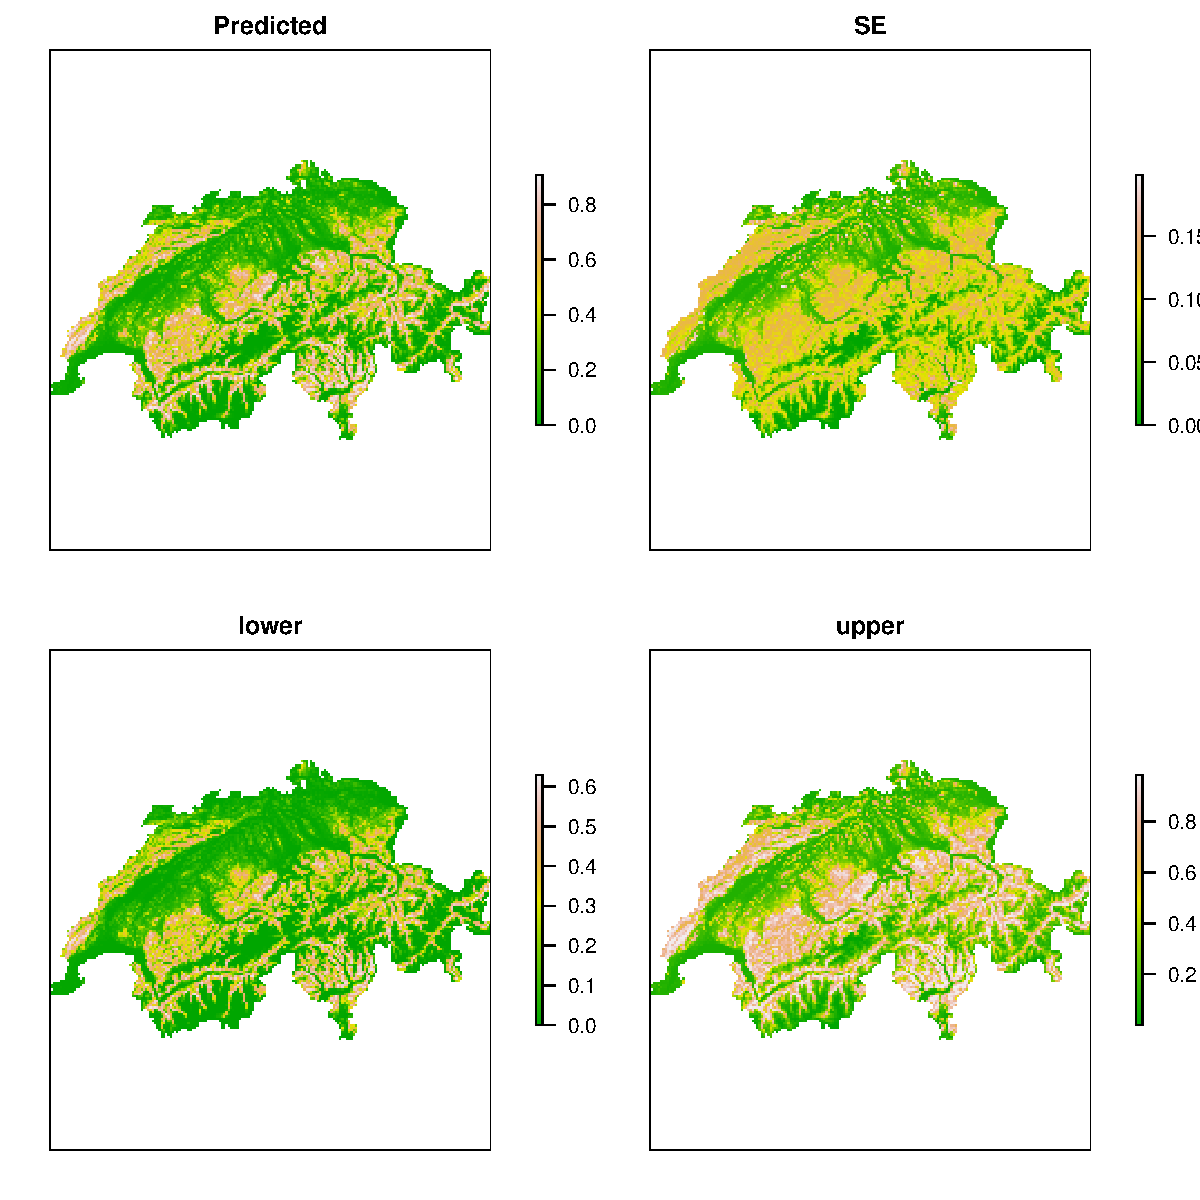
\includegraphics[width=5in,height=5in]{spp-dist-psi2}
\caption{Expected occurrence probability along with standard errors
  and the limits of the asymptotic 95\% confidence interval.}
\label{fig:predict}
\end{figure}

Users should be cautious when predicting from models that have
categorical predictor variables, \emph{i.e.} \verb+factor+s. The
\texttt{raster} package does not have advanced methods for handling
factors, and thus it is not easy to automatically create dummy
variables from them as can typically be done using
\verb+model.matrix+. The safest option is to create the dummy
variables manually before fitting the models, and to use the same
variables as rasters for prediction.

A more important consideration when creating species distribution maps
based upon occurrence probability is that of spatial scale. Occurrence
probability will typically depends upon the area of the ``site'' in
question. Thus, in our crossbill example, it would not be appropriate
to use our model to predict occcurrence probability for 10-km$^2$
pixels since the surveys were done in 1-km$^2$ quadrats. In some
cases it might be possible to directly model the effect of site area
on occurrence probability, in which case the effect could be accounted
for in the predictions.

\section*{Mapping Population Density}

Although distribution is typically described in terms of
ocurrence probability, which is always better than an index of
occurrence probability, the best parameter for modeling species
distribution is population density because density allows for
inference about popualation size in an region of
the species' range. Furthermore, occurrence probability is simply the
probablity that abundance is greater than 0, so with density/abundance
estimates, it is always possible to compute occurrence probablity as a
derived parameter.

In this example, we create a distribution map for the Island Scrub-Jay
(\textit{Aphelocoma insularis}), which is restricted to Santa Cruz
Island, California. To do so, we fit the hierarchical distance
sampling model of \citet{royle_modeling_2004}, which allows for the
estimation of abundance in each of the $300 \times 300$m pixels
representing the island. The data were collected 307, 300-m radius
point count (or ``point transect'') surveyed during the Fall of 2008.

{\color{red} Important} This analysis is for demonstration
purposes only, and the estimates of population size should not be used
for conservation or management purposes. Indeed, the Poisson
assumption used here was found to be inadequate by
\citet{sillett_etal:2012} who conducted a rigorous analysis and
reported reliable estimate of population size.

Although we are fitting a model of population density, the steps of
the analysis closely mirror those shown in the previous
section. First, we format the data and fit a model, then we format the
island-wide covariates and make predictions. The three covariates
thought to influence jay abundance are elevation, forest cover, and
chapararral cover. We also include include the area of the survey
plots in the analysis so that we can make predictions for regions of
any area. Here is the code to format the data and fit the model.

\begin{Schunk}
\begin{Sinput}
> data(issj)
> covs <- scale(issj[,c("elevation", "forest", "chaparral")])
> area <- pi*300^2 / 10000
> jayumf <- unmarkedFrameDS(y=as.matrix(issj[,1:3]),
                           siteCovs=data.frame(covs, area),
                           dist.breaks=c(0,100,200,300),
                           unitsIn="m", survey="point")
> head(jayumf)
\end{Sinput}
\begin{Soutput}
Data frame representation of unmarkedFrame object.
   y.1 y.2 y.3   elevation     forest  chaparral     area
1    0   0   2 -1.20607849 -0.3309618 -0.1218243 28.27433
2    0   0   0 -0.36132054 -0.4429552  0.8384709 28.27433
3    0   0   0 -0.45797193 -0.3738751  2.1319298 28.27433
4    0   0   0 -0.14196112  1.3908065 -0.2737078 28.27433
5    0   0   0 -0.72588125 -0.4869152 -1.1562240 28.27433
6    0   0   0  0.01704522  0.6706992  0.2989173 28.27433
7    0   0   0 -0.11866710 -0.2671150  1.0326122 28.27433
8    0   0   0 -0.76411740 -0.4921486 -0.9332983 28.27433
9    0   0   0  0.40065595  0.5440524 -1.0759952 28.27433
10   0   0   0 -0.24030211 -0.4921486 -1.1023299 28.27433
\end{Soutput}
\begin{Sinput}
> fm1 <- distsamp(~chaparral ~chaparral + elevation + offset(log(area)),
                 jayumf, keyfun="halfnorm", output="abund",
                 starts=c(-2.8,1,0,4.5,0))
> fm1
\end{Sinput}
\begin{Soutput}
Call:
distsamp(formula = ~chaparral ~ chaparral + elevation + offset(log(area)), 
    data = jayumf, keyfun = "halfnorm", output = "abund", starts = c(-2.8, 
        1, 0, 4.5, 0))

Abundance:
            Estimate     SE      z  P(>|z|)
(Intercept)   -2.827 0.1609 -17.57 4.34e-69
chaparral      0.957 0.1460   6.55 5.60e-11
elevation     -0.244 0.0932  -2.61 8.96e-03

Detection:
                 Estimate     SE     z  P(>|z|)
sigma(Intercept)     4.73 0.0845 55.96 0.000000
sigmachaparral      -0.25 0.0744 -3.36 0.000773

AIC: 964.6426 
\end{Soutput}
\end{Schunk}

Remarks. 1) The distance data were binned into 3 distance classes. 2)
We used \verb+output="abund"+ even though, by specifying the offset,
we effectively modeled population density. As stated previously, this
allows us to make predictions of abundance for regions of arbitrary size.



\begin{comment}

\begin{Schunk}
\begin{Sinput}
> data(issj)
> data(cruz)
> elev <- rasterFromXYZ(cruz[,c("x","y","elevation")],
      crs="+proj=utm +zone=11 +ellps=GRS80 +datum=NAD83 +units=m +no_defs")
> #plot(elev, col=terrain.colors(100))
> #points(issj[,c("x","y")], cex=0.5)
\end{Sinput}
\end{Schunk}
\includegraphics{spp-dist-011}
print(
wireframe(elevation ~ x + y, cruz, drape=TRUE,
          screen=list(z=10, x=-10),
          aspect=0.5, xlab="", ylab="", zlab="",
#          xlim=c(229900,267000), ylim=c(3762000,3770000),
          par.settings = list(axis.line = list(col = "transparent")),
          par.box = c(col = "transparent"),
          col.regions=terrain.colors(100),
          colorkey=FALSE)
)

\end{comment}


The next thing to do is to format the raster data. For details, see
the previous section---the process is the same, except that we need a
raster for ``area'', the size of each pixel in the raster data. This
is necessary because the survey plots were larger than the pixels for
which we want predictions of abundance.

\begin{Schunk}
\begin{Sinput}
> data(cruz)
> elev <- rasterFromXYZ(cruz[,c("x","y","elevation")],
      crs="+proj=utm +zone=11 +ellps=GRS80 +datum=NAD83 +units=m +no_defs")
> forest <- rasterFromXYZ(cruz[,c("x","y","forest")],
      crs="+proj=utm +zone=11 +ellps=GRS80 +datum=NAD83 +units=m +no_defs")
> chap <- rasterFromXYZ(cruz[,c("x","y","chaparral")],
      crs="+proj=utm +zone=11 +ellps=GRS80 +datum=NAD83 +units=m +no_defs")
> area.raster <- chap
> values(area.raster) <- 300*300/10000 # area of a grid pixel
> attr(covs, "scaled:center")
\end{Sinput}
\begin{Soutput}
  elevation      forest   chaparral 
202.0023616   0.0673357   0.2703592 
\end{Soutput}
\begin{Sinput}
> attr(covs, "scaled:scale")
\end{Sinput}
\begin{Soutput}
  elevation      forest   chaparral 
124.8818069   0.1368199   0.2338295 
\end{Soutput}
\begin{Sinput}
> elev.s <- (elev-202)/125
> forest.s <- (forest-0.0673)/0.137
> chap.s <- (chap-0.270)/0.234
> habitat <- stack(elev.s, forest.s, chap.s, area.raster)
> layerNames(habitat) <- c("elevation", "forest", "chaparral", "area")
\end{Sinput}
\end{Schunk}


Now, when we use \verb+predict+, it will return the expected number of
jays in each pixel along with the standard errors and the 95\%
confidence intervals. We could sum these up to obtain an estimate of
total population size. \citet{sillett_etal:2012} did this and used the
parametric boostrap to estimate the variance of total population
size.

\begin{Schunk}
\begin{Sinput}
> E <- predict(fm1, type="state", newdata=habitat)
\end{Sinput}
\begin{Soutput}
  doing row 1000 of 5625 
  doing row 2000 of 5625 
  doing row 3000 of 5625 
  doing row 4000 of 5625 
  doing row 5000 of 5625 
\end{Soutput}
\begin{Sinput}
> plot(E, axes=FALSE, col=terrain.colors(100))
\end{Sinput}
\end{Schunk}
\begin{figure}
  \centering
\includegraphics[width=6in,height=5in]{spp-dist-issj}
\caption{Expected Island Scrub-Jay abundance, SEs, and 95\% CIs.}
\label{fig:issj}
\end{figure}







\newpage

\bibliography{unmarked}

\end{document}
